\section{Budget}



% =======================================================================================
% =======================================================================================
% =======================================================================================
% =======================================================================================
% Revenue Section
% =======================================================================================
% =======================================================================================
% =======================================================================================
% =======================================================================================

\subsection{Revenue}
We have compared the predicted and actual revenues from previous reports and used these to estimate our expected revenue. To maintain reasonable accuracy in the budget, we were financially conservative in our estimates to account for fluctuating economy and attendance numbers. Should our bid be selected, these conservative estimates will result in a smoother planning and execution process. We have also accounted an estimated number of waived professional registration based on previous conferences. This  correlates to the number of waived fees given in our expected tier sponsorship figures and also factors in discounts to speakers, panelists, and workshop instructors. \\

\begin{table}[H]
\centering
\caption*{\textbf{Attendance}}
\begin{tabular}{|c|c|c|c|}
\hline
    \textbf{Item} & \textbf{Quantity} & \textbf{Cost} & \textbf{Subtotal}	\\ 
\hline
	Student			&	443	&	\$40	&	\$17,720						\\
	Professional	&	127	& 	\$250	&	\$31,750						\\
	Waived			&	60	& 	-\$250	&	-\$15,000						\\
\hline
	\multicolumn{3}{|r|}{\textbf{Attendance Total:}}	&	\$34,470		\\
\hline
\end{tabular}
\end{table}

\vspace{10mm}

\begin{table}[H]
\centering
\caption*{\textbf{Sponsors}}
\begin{tabular}{|c|c|c|c|}
\hline
    \textbf{Package} & \textbf{Quantity} & \textbf{Cost} & \textbf{Subtotal}	\\ 
\hline
	World Savior	&	1	&	\$30,000	&	\$30,000						\\
	National Hero	&	3	& 	\$15,000	&	\$45,000						\\
	Local Prodigy	&	5	& 	\$10,000	&	\$50,000						\\
	Lifesaver		&	6	& 	\$5,000		&	\$30,000						\\
	Exhibitor+		&	3	& 	\$3,500		&	\$10,500						\\
	Exhibitor		&	5	& 	\$2,500		&	\$12,500						\\
	Good Samaritan	&	10	& 	\$1,500		&	\$15,000						\\
	Contributor		&	8	& 	\$1,000		&	\$8,000							\\
\hline
	\multicolumn{3}{|r|}{\textbf{Sponsors Total:}}	&	\$201,000				\\
\hline
\end{tabular}
\end{table}

\vspace{10mm}

\begin{table}[H]
\centering
\begin{tabular}{|c|}
\hline
    \textbf{Total Revenue: \$235,470}\\ 
\hline
\end{tabular}
\end{table}

% =======================================================================================
% =======================================================================================
% =======================================================================================
% =======================================================================================
% Expenses Section
% =======================================================================================
% =======================================================================================
% =======================================================================================
% =======================================================================================

\subsection{Expenses}
A conservative breakdown of conference expenses is outlined in Table ******* on page *******. Emphasizing some of the points shown in the table, all rooms hosted in the Union are provided to registered student organizations (such as ANS) free of charge, which allows us to save significantly on event space. Gratuity is omitted for all catering provided by the University Catering service, as the University is unable to accept gratuity on purchases. 
Under our most conservative estimates for budget and revenue, the spending margin is found to be 9.62\%. This margin is generous and in line with that allotted in previous years. Additionally, our budget calls for significantly higher student travel reimbursements than what where accounted for in previously proposed budgets. Reducing to levels proposed in recent years would free an additional $\$$ 40,000, if absolutely necessary. 
Assuming maximum expenses and an attendance of 450 students, the total cost per student is estimated at \$ 485.05. This number also includes the travel reimbursement, which was intentionally set to be considerably more generous than previous years to make the budget more conservative. Neglecting the cost of travel reimbursements, the average cost per student falls to \$260.05, at or below that estimated for previous years. 

\hspace{-1.1cm}
\begin{tabular}{|clcrccccr|}

    \hline
     & \multicolumn{1}{c}{Item} & \multicolumn{1}{c}{Priority} & \multicolumn{1}{c}{Cost Per Unit} & \multicolumn{1}{c}{Thursday} & \multicolumn{1}{c}{Friday} & \multicolumn{1}{c}{Saturday} & \multicolumn{1}{c}{General} & \multicolumn{1}{c}{Total Cost}\\     \hline\hline
     \multirow{12}{*}{\STAB{\rotatebox[origin=c]{90}{Facilities}}}
     & Technical Session AV      & I                         & $\$$ 13.80                & 1                         & 7                        & 7                         & -                         & $\$$ 207.00               \\
     & Technical Session Rooms   & I                         & $\$$ 0.00                 & -                         &  -                       &  -                        &  1                        & $\$$ 0.00                 \\
     & Panel AV                  & I                         & $\$$ 17.80                & -                         &   2                      &   2                       &   -                       & $\$$ 71.20                \\ 
     & Panel Rooms               & I                         & $\$$ 0.00                 & -                         &    -                     &    -                      &    1                      & $\$$ 0.00                 \\
     & Workshop AV               & I                         & $\$$ 17.80                & 2                         &     -                    &     -                     &     -                     & $\$$ 35.60                \\
     & Workshop Rooms            & I                         & $\$$ 0.00                 &  -                        &      -                   &      -                    &      1                    & $\$$ 0.00                 \\ 
     & Dinner Room (Garden)      & I                         & $\$$ 4,000.00             &   1                       &       -                  &       -                   &       -                   & $\$$ 4,000.00             \\
     & Dinner AV (Garden)        & I                         & $\$$ 0.00                 &    1                      &        -                 &        -                  &        -                  & $\$$ 0.00                 \\
     & Dinner Room (I-Hotel)     & I                         & $\$$ 4,000.00             &     -                     &         1                &         -                 &         -                 & $\$$ 4,000.00             \\ 
     & Dinner AV (I-Hotel)       & I                         & $\$$ 0.00                 &      -                    &          1               &          -                &          -                & $\$$ 0.00                 \\
     & Dinner Room (Union)       & I                         & $\$$ 0.00                 &     -                     &         -                &         1                 &         -                 & $\$$ 0.00                 \\ 
     & Dinner AV (Union)         & I                         & $\$$ 17.80                &      -                    &          -               &        1                  &          -                & $\$$ 17.80                \\ \hline  
     
     &                           &                           &                           &                           &\multicolumn{3}{r}{Facilities Subtotal:}     & $\$$ 8,331.60            \\ \hline\hline
     \multirow{10}{*}{\STAB{\rotatebox[origin=c]{90}{Transport}}}
     & Shuttles From Hotel       & I                         & $\$$ 1,000.00             & 4                         & 4                        & 4                         & -                         & $\$$ 12,000.00            \\
     & Ihotel Dinner             & I                         & $\$$ 100.00               & -                         &  4                       &  -                        &  -                        & $\$$ 400.00               \\
     & Union Dinner              & I                         & $\$$ 100.00               & -                         &   -                      &   4                       &   -                       & $\$$ 400.00               \\
     & Barn Dance/Ice Skating    & III                       & $\$$ 300.00               & 4                         & -                        & -                         & -                         & $\$$ 1,200.00             \\
     & Memorial Stadium Social   & III                       & $\$$ 300.00               & -                         &  4                       &  -                        &  -                        & $\$$ 1,200.00             \\
     & Downtown Champaign Social & III                       & $\$$ 300.00               & -                         &   -                      &   4                       &   -                       & $\$$ 1,200.00             \\
     & Triptych/Blue Waters Tour & II                        & $\$$ 875.00               & 1                         &   -                      &   -                       &   -                       & $\$$ 875.00               \\ 
     & Riggs Tour                & III                       & $\$$ 875.00               & 1                         &    -                     &    -                      &    -                      & $\$$ 875.00               \\
     & Clinton Tour              & II                        & $\$$ 900.00               & 1                         &    -                     &    -                      &    -                      & $\$$ 900.00               \\
     & Argonne Tour              & II                        & $\$$ 900.00               & 1                         &     -                    &     -                     &     -                     & $\$$ 900.00               \\ \hline
     &                           &                           &                           &                           &\multicolumn{3}{r}{Transport Subtotal:}      & $\$$ 19,950.00            \\ \hline\hline
     \multirow{6}{*}{\STAB{\rotatebox[origin=c]{90}{Food}}}
     & Coffee/Tea                & II                        & $\$$ 1.95                 & -                         & 600                      & 600                       & -                         & $\$$ 2,340.00             \\
     & Garden Hotel Dinner       & II                        & $\$$ 36.50                & 600                       & -                        &  -                        &  -                        & $\$$ 26,280.00            \\
     & Ihotel Dinner             & II                        & $\$$ 27.50                & -                         &   600                    &   -                       &   -                       & $\$$ 16,500.00            \\ 
     & Union Dinner              & II                        & $\$$ 27.50                & -                         &   -                      &   600                     &   -                       & $\$$ 16,500.00            \\
     & Dinner Cash Bars          & III                       & $\$$ 336.00               & 1                         &    1                     &    1                      &    -                      & $\$$ 1,008.00             \\
     & SSC Lunches               & II                        & $\$$ 16.50                & -                         &     -                    &     150                   &     -                     & $\$$ 2,475.00             \\ \hline
     &                           &                           &                           &                           &\multicolumn{3}{r}{Food Subtotal:}           & $\$$ 65,103.00            \\ \hline\hline
     \multirow{5}{*}{\STAB{\rotatebox[origin=c]{90}{Socials}}}
     & Ice Skating               & III                       & $\$$ 240.00               & 2                         & -                        & -                         & -                         & $\$$ 480.00               \\
     & Barn Dance                & IV                        & $\$$ 2,800.00             &  1                        & -                        &  -                        &  -                        & $\$$ 2,800.00             \\
     & Memorial Stadium Club 77  & III                       & $\$$ 2,000.00             & -                         &   1                      &   -                       &   -                       & $\$$ 2,000.00             \\ 
     & Club 77 Tab               & IV                        & $\$$ 2,000.00             & -                         &    1                     &    -                      &    -                      & $\$$ 2,000.00             \\
     & Guido's Tab               & IV                        & $\$$ 2,000.00             & -                         &     -                    &     1                     &     -                     & $\$$ 2,000.00             \\ \hline
     &                           &                           &                           &                           &\multicolumn{3}{r}{Socials Subtotal:}        & $\$$ 9,280.00             \\ \hline\hline
     \multirow{8}{*}{\STAB{\rotatebox[origin=c]{90}{Miscellaneous}}}
     & Conference Programs       & I                         & $\$$ 2,133.90             & -                         & -                        & -                         & 1                         & $\$$ 2,133.90             \\
     & Lanyards                  & I                         & $\$$ 2.54                 &  -                        & -                        &  -                        &  600                      & $\$$ 1,524.00             \\
     & Award Certificates        & II                        & $\$$ 2.50                 & -                         &   -                      &   50                      &   -                       & $\$$ 125.00               \\ 
     & Poster Session Prizes     & II                        & $\$$ 100.00               & -                         &    -                     &    3                      &    -                      & $\$$ 300.00               \\
     & Swag                      & IV                        & $\$$ 10,000.00            & -                         &     -                    &     -                     &     1                     & $\$$ 10,000.00            \\ 
     & Triptych Tour             & III                       & $\$$ 5.00                 & 55                        &     -                    &     -                     &     -                     & $\$$ 275.00               \\
     & Riggs Tour                & III                       & $\$$ 0.00                 & 55                        &     -                    &     -                     &     -                     & $\$$ 0.00                 \\
     & Travel Reimbursements     & I                         & $\$$ 225.00               &  -                        &     -                    &                           &  450                      & $\$$ 101,250.00           \\ \hline
     &                           &                           &                           &                           &\multicolumn{3}{r}{Miscellaneous Subtotal:}                                       & $\$$ 115,607.90           \\ \hline\hline
     &                           &                           &                           &                           &                          &                           &                           &                           \\
     &                           &                           &                           &                           &\multicolumn{3}{r}{Grand Total:}                                                  & $\$$218,272.50            \\
     &                           &                           &                           &                           &                          &                           &                           &                           \\ \hline
\end{tabular}

\subsection{Financial Contingency}


\begin{tabular}{lrrr}
  \hline\hline
  \multicolumn{1}{l}{Level of Cuts Made} & \multicolumn{1}{c}{Amount Saved} & \multicolumn{1}{c}{Grand Total} & \multicolumn{1}{c}{\% Margin} \\ \hline\hline 
  Priority IV Cuts Made & $\$$ 9,800.00 & $\$$ 208,472.50 & 13.68 \% \\
  III and IV Cuts Made & $\$$ 23,648.00 &$\$$ 194,624.50 & 19.41 \% \\
  II, III, and IV Cuts Made & $\$$ 40,393.00 & $\$$ 177,879.50 & 26.34 \% \\
  
  \end{tabular}

The budget is structured with priority levels outlining the order of cuts, should they be necessary. Priority I expenses are not subject to cuts under any circumstances as they are considered necessities for hosting the conference. Cuts will be made first to reduce most priority IV expenses by half, preserving events while still saving money. Priority III cuts mean eliminating all priority IV expenses and either elimination of, or reduction of the duration of social events by half. Priority II cuts entail complete elimination of social event expenses, along with elimination of tour expenses and reduction of dinner costs through cheaper buffet options and desserts. The expenditure savings from these cuts are outlined in Table *******. While this contingency plan does not consider cuts to the reimbursement funds, this could be reconsidered if necessary, since reimbursements were set aside at a level nearly double that of previous conferences. \\

\subsection{Sponsorship and Fundraising}
The sponsorship breakdown for our conference pulls from averages of sponsorship packages in the last several conferences, with for main tiers that tie into the conference theme for the largest representation in the conference and visibility in the career fair, socials, sessions, technical, and meals as well as in conference shirts and attendee bags. Using two tiers for an exhibitor package allows for a platform for DOE national laboratories to participate, with the higher tier having logo representation on shirts as well as the opportunity to sponsor a coffee break or lunch \& learn session. Lastly, two packages are left to benefactors who are recognized in the conference program and represent the anticipated support from ANS divisions or local industry or University of Illinois contributors (or some generous contributions from out-of-state companies!). 

\vspace{1cm}

\begin{figure}[H]
	\centering
	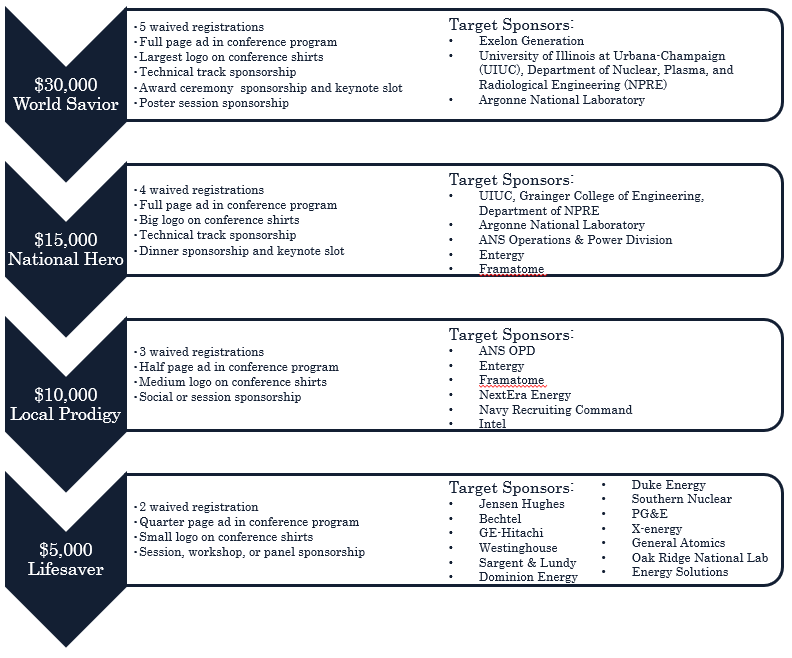
\includegraphics[width=\textwidth]{sponsors1.png}	
\end{figure} 

\begin{figure}[H]
	\centering
	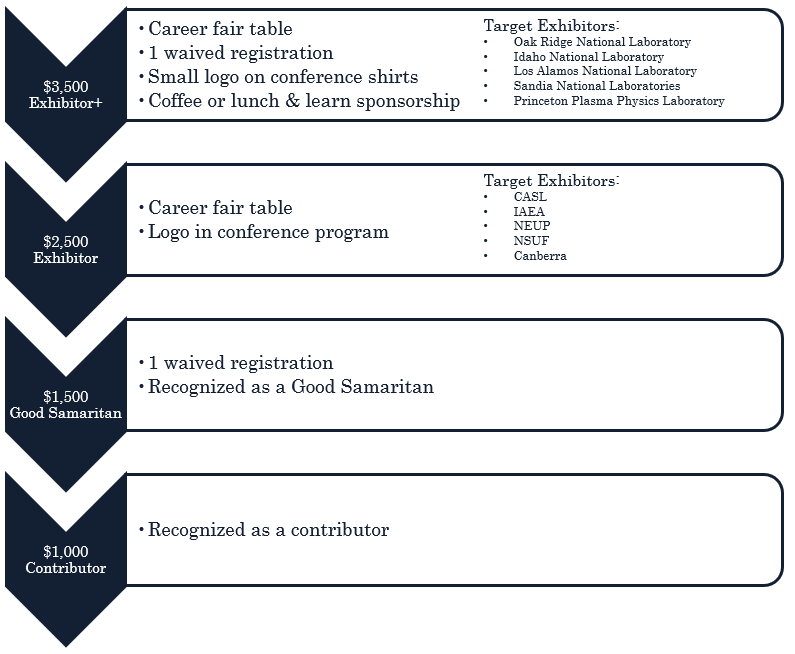
\includegraphics[width=\textwidth]{sponsors2.png}	
\end{figure} 

\subsection{Banking}

In order to properly handle all of the conference expenses, two accounts will be used. One account will be with the national ANS headquarters, and the second will be a local checking account through Busey Bank. Our student section currently holds a checking account with Busey Bank and has developed a working relationship with them. Similar to previous conferences, the national ANS account will be the primary account due to their previous experience in handling conference funds and their 501(c)(3) tax exemption status. Although an account with the national ANS organization is currently not maintained by the UIUC local chapter, should this bid be selected, the opening of an account would happen almost immediately. An established local checking account with Busey Bank allows for convenience when using them as a secondary account. The student section account has been maintained for a number of years, allowing for adequate knowledge of Busey’s policies and a stable relationship to be established with the local branch. A new account would be opened, such that the student chapter funds and the conference funds are completely separate and require different oversight. This account will be used for small expenses that can occur during the conference. Although the ANS-managed account could be used for such purposes, the presence of a local branch allows for more flexibility if a purchase becomes time sensitive. Should the additional Busey Bank account be unobtainable, an account would be established with Chase instead. If ANS National desires to manage all funds, accommodations will be made to consolidate the funds.

\subsubsection{Financial Oversight}
Financial integrity must be maintained when providing a conference of this size. To do so, diligent oversight will be practiced for all transactions related to the conference. Expense requests will be required for all transactions. These requests must carefully outline the reason for the purchase and the total cost. If the purchase is reoccuring, automation will be required at the time of request. These requests will require the approval of both conference chairs in addition to the financial director. Only the conference chairs and the financial director will have authority, assuming the previously mentioned permission, to complete transactions on the Busey Bank account. To ensure transparency, the financial director will update a public record containing all transactions. 

\subsection{Cost of Attendance and Student Reimbursement}
The cost of attending the student conference, per student, varies among schools and is highly dependent on distance from UIUC and the preferred mode of travel. We will assume that minimizing cost is a priority for schools, thus number of persons per hotel room is double the number of beds. The University of Illinois is a 2.5 hour drive from one of the largest airports in the world, O'Hare International Airport. There is also a small airport located just 20 minutes outside of campus. Additionally, there is a reliable bus service, Peoria Charter, that runs between O'Hare and the UIUC campus up to 10 times per day. Below are the round-trip, non-stop, airfare costs for the first weekend of April. Peoria Charter fare from O'Hare to UIUC is currently $\$61$ round-trip. While some students may wish to make use of the convenience of the local airport, in general the most economic method of arriving in Champaign is by first flying to O’Hare and then busing. The average cost of this trip comes out to be \$293 as shown in Table *******. Adding this to the registration and lodging costs for four nights (as students often arrive Wednesday evening) and assuming four students per room, the total cost of attendance for each student comes out to an average of \$447.

% Jeremy's budget plan
